% EJC papers *must* begin with the following two lines. 
\documentclass[12pt]{article}
\usepackage{e-jc}

% Please remove all other commands that change parameters such as
% margins or pagesizes.

% only use standard LaTeX packages
% only include packages that you actually need
\usepackage{enumerate}

% we recommend these ams packages
\usepackage{amsthm,amsmath,amssymb}

% we recommend the graphicx package for importing figures
\usepackage{graphicx}

% use this command to create hyperlinks (optional and recommended)
\usepackage[colorlinks=true,citecolor=black,linkcolor=black,urlcolor=blue]{hyperref}

%%%% REMOVE FOR FINAL DRAFT: %%%%
%\usepackage{showkeys}
%\usepackage[left=2in, right=2in]{geometry}

% use these commands for typesetting doi and arXiv references in the bibliography
\newcommand{\doi}[1]{\href{http://dx.doi.org/#1}{\texttt{doi:#1}}}
\newcommand{\arxiv}[1]{\href{http://arxiv.org/abs/#1}{\texttt{arXiv:#1}}}

% all overfull boxes must be fixed; 
% i.e. there must be no text protruding into the margins

% declare theorem-like environments
\theoremstyle{plain}
\newtheorem{theorem}{Theorem}
\newtheorem{lemma}[theorem]{Lemma}
\newtheorem{corollary}[theorem]{Corollary}
\newtheorem{proposition}[theorem]{Proposition}
\newtheorem{fact}[theorem]{Fact}
\newtheorem{observation}[theorem]{Observation}
\newtheorem{claim}[theorem]{Claim}

\theoremstyle{definition}
\newtheorem{definition}[theorem]{Definition}
\newtheorem{example}[theorem]{Example}
\newtheorem{conjecture}[theorem]{Conjecture}
\newtheorem{open}[theorem]{Open Problem}
\newtheorem{problem}[theorem]{Problem}
\newtheorem{question}[theorem]{Question}

\theoremstyle{remark}
\newtheorem{remark}[theorem]{Remark}
\newtheorem{note}[theorem]{Note}

% custom markup
\DeclareMathOperator*{\spec}{Spec}
\DeclareMathOperator*{\tr}{tr}
\providecommand{\cover}[1]{\widetilde{#1}}
\providecommand{\rev}[1]{\bar{#1}}
\providecommand{\abs}[1]{\lvert #1 \rvert}

%%%%%%%%%%%%%%%%%%%%%%%%%%%%%%%%%%%%%%%%%%%%%%%%%%%%%%%

% if needed include a line break (\\) at an appropriate place in the title

\title{\bf Orbigraphs: Defining a Graph Theoretic Analog to Reimannian Orbifolds}

% input author, affilliation, address and support information as follows;
% the address should include the country, and does not have to include
% the street address 

\author{Dr. Liz Stanhope\\
\small Department of Mathematical Sciences\\[-0.8ex]
\small Lewis and Clark College\\[-0.8ex] 
\small Portland, Oregon\\
\small\tt lstanhope@lclark.edu\\
% \and
% Forgotten Second Author \qquad  Forgotten Third Author\\
% \small School of Hard Knocks\\[-0.8ex]
% \small University of Western Nowhere\\[-0.8ex]
% \small Nowhere, Australasiaopia\\
% \small\tt \{fsa,fta\}@uwn.edu.ao
}

% \date{\dateline{submission date}{acceptance date}\\
% \small Mathematics Subject Classifications: comma separated list of
% MSC codes available from http://www.ams.org/mathscinet/freeTools.html}

\date{\dateline{July 29, 2013}{July 29, 2013}\\
\small Mathematics Subject Classifications: 05C88, 05C89}

\begin{document}

\maketitle

% E-JC papers must include an abstract. The abstract should consist of a
% succinct statement of background followed by a listing of the
% principal new results that are to be found in the paper. The abstract
% should be informative, clear, and as complete as possible. Phrases
% like "we investigate..." or "we study..." should be kept to a minimum
% in favor of "we prove that..."  or "we show that...".  Do not
% include equation numbers, unexpanded citations (such as "[23]"), or
% any other references to things in the paper that are not defined in
% the abstract. The abstract will be distributed without the rest of the
% paper so it must be entirely self-contained.

%%%%%%%%%%%%%%%%%%%%%%%%%%%%%%%%%%%%%%%%%%%%%%%%%%%%%%%
\begin{abstract}
Riemannian orbifolds are a slight generalization of Riemannian manifolds.  Instead of being locally diffeomorphic to $\mathbb{R}^n$, Riemannian orbifolds are locally diffeomorphic to $\mathbb{R}^n$ modulo the isometric action of a finite group.  Recently, a number of authors have examined orbifolds from the perspective of inverse spectral geometry.  In light of the strong connection between spectral geometry and spectral graph theory, our project defines a graph theoretic parallel of an orbifold, called an orbigraph, and obtains spectral results about orbigraphs.  The graph theoretic analogue of a manifold is taken to be a $k$-regular graph.  Because the local structure of a $k$-regular graph is a $k$-star, we form a $k$-orbigraph by patching together quotients of $k$-stars.  The resulting class of objects (the $k$-orbigraphs) consists of directed multigraphs satisfying certain outdegree conditions.  The spectrum of the adjacency matrix of a $k$-orbigraph yields bounds on the number of singular (non $k$-star) vertices present in the orbigraph.  The reversibility (as in Markov chains) of an orbigraph determines if it can be obtained as the quotient of a finite $k$-regular graph.  Our methods include computational algorithms and formal graph theoretic arguments.  Both the definition of an orbigraph and our results about them are new.

  % keywords are optional
  \bigskip\noindent ``All perception of truth is the perception of an analogy.'' -- \textit{Thoreau}
  % Nothing is either good or bad but by comparison (Anonymous)
  % Bad is called good when worse happens (Anonymous)

\end{abstract}


%%%%%%%%%%%%%%%%%%%%%%%%%%%%%%%%%%%%%%%%%%%%%%%%%%%%%%%
\section{Introduction}

  How exciting can we make the intro without sound too informal?
  Introduction describing motivation
  Introduce project; describe student contributions over multiple summers?

  

  %%%%%%%%%%%%%%%%%%%%%%%%%%%%%%%%%%%%%%%%%%%%%%%%%%%%%%%
  \subsection{Notation}
  Let $\Gamma$ be a graph, possibly directed with multiple edges. Its vertex set will be denoted $V(\Gamma)$ and its edge set $E(\Gamma)$. Furthermore, if $u, v \in V(\Gamma)$, then $w_\Gamma(u, v)$ will denote the number of edges from $u$ to $v$. In cases when the context is clear, this notation may be abbreviated to $w(u,v)$. Then for an enumeration $v_1, \ldots, v_n$ of $V(\Gamma)$, the adjacency matrix $A(\Gamma)$ is given by $A(\Gamma)_{ij} = w_\Gamma(v_i, v_j)$. If $e \in E(\Gamma)$ then $o(e)$ denotes the origin of the edge and $t(e)$ denotes its terminus. A walk in $\Gamma$ is a sequence of edges $e_1,\ldots,e_n$ such that $t(e_i) = o(e_{i+1})$ for $1 \le i < n$. A walk is closed if $o(e_1) = t(e_n)$. A closed walk may be referred to as a loop at $o(e_1)$.

  Also, note that the adjacency matrix can be viewed as a linear operator on the function space $\mathbb{C}^{V(\Gamma)}$. This operator will be denoted $A_\Gamma$ and is defined for $\psi \in \mathbb{C}^V(\Gamma)$ and $v \in V(\Gamma)$ by
  $$
    [A_\Gamma \psi](v) = \sum_{u \in V(\Gamma)} w(v, u)\psi(u).
  $$


%%%%%%%%%%%%%%%%%%%%%%%%%%%%%%%%%%%%%%%%%%%%%%%%%%%%%%%
\section{Brief introduction to Riemannian orbifolds}

  Brooks analogy, Bass Serre Theory mention.


%%%%%%%%%%%%%%%%%%%%%%%%%%%%%%%%%%%%%%%%%%%%%%%%%%%%%%%
\section{Defining Orbigraphs as Analogs of Orbifolds}

  Reasons for choices, etc.

  \begin{definition}\label{def:OrbigraphDefn}
    A \textbf{$k$-orbigraph} is a directed graph $\Gamma$ where the adjacency matrix $A(\Gamma)$ satisfies the following:
    
    \begin{enumerate}[i.]
      \item $A(\Gamma)_{ij} \in \mathbb{Z}_{\ge 0}$
      \item $\sum_j A(\Gamma)_{ij} = k$
      \item $A(\Gamma)_{ij} > 0$ if and only if $A(\Gamma)_{ji} > 0$.
    \end{enumerate}

  \end{definition}


%%%%%%%%%%%%%%%%%%%%%%%%%%%%%%%%%%%%%%%%%%%%%%%%%%%%%%%
\section{Properties of Orbigraphs}


  %%%%%%%%%%%%%%%%%%%%%%%%%%%%%%%%%%%%%%%%%%%%%%%%%%%%%%%
  \subsection{Covering Theory for Orbigraphs}

    Start with covering theory because it lets us characterize orbigraphs as quotients of $k$-trees by equitable partitions.

    \begin{definition}\label{def:EqPartitionDefn}
      Let $\Gamma$ be an orbigraph and $\pi = \{ \pi_1, \ldots, \pi_m \}$ be a partition of its vertices. Then $\pi$ is an \textbf{equitable partition} if for $v \in \pi_i$, the number $A(\Gamma / \pi)_{ij} = \sum_{u \in \pi_j} w(v, u)$ is independent of the choice of $v$. The multi-digraph with adjacency matrix $A(\Gamma / \pi)$ is called the \textbf{quotient graph}.
    \end{definition}

    \begin{lemma}\label{lemma:EqPartitionQuotient}
      If $\Gamma$ is an $k$-orbigraph and $\pi$ is an equitable partition of $\Gamma$, then $\Gamma / \pi$ is a $k$-orbigraph.
    \end{lemma}
    \begin{proof}
      Because $\Gamma$ is an orbigraph, we have $w_\Gamma(v, u) \in \mathbb{Z}_{\ge 0}$ for all $u, v \in V(\Gamma)$. Hence, $A(\Gamma / \pi)_{ij} = \sum_{u \in \pi_j} w_\Gamma(v, u) \in \mathbb{Z}_{\ge 0}$ for any $v \in \pi_i$. Now let $v \in \pi_i$ so we have
      
      \begin{align*}
        \sum_j A(\Gamma / \pi)_{ij} &= \sum_j \sum_{u \in \pi_j} w_\Gamma(v, u) \\
        &= \sum_{u \in \Gamma} w_\Gamma(v, u) = k.
      \end{align*}

      Finally, assume that $A(\Gamma / \pi)_{ij} > 0$. Then there must be a $u \in \pi_j$ for some $j$ such that $w_\Gamma(v, u) > 0$. Because $\Gamma$ is an orbigraph, we must have $w_\Gamma(u, v) > 0$. Thus $A(\Gamma / \pi)_{ji} > 0$.
    \end{proof}

    We say that an orbigraph $\Gamma_1$ covers an orbigraph $\Gamma_2$ if there is an equitable partition $\pi$ of $\Gamma$ such that $\Gamma_1 / \pi = \Gamma_2$.

    \begin{lemma}\label{lemma:CoveringTransitivity}
      The covering relation is transitive.
    \end{lemma}
    \begin{proof}
      We wish to show that if $\Gamma_1$ is an orbigraph with equitable partition $\pi_1$ such that $\Gamma_1 / \pi_1 = \Gamma_2$ and $\Gamma_2$ has an equitable parition $\pi_2$ such that $\Gamma_2 / \pi_2 = \Gamma_3$, then there is an equitable partition $\pi_1 \circ \pi_2$ of $\Gamma_1$ such that $\Gamma_1 / (\pi_1 \circ \pi_2) = \Gamma_3$. Denote the partition matrix associated with equitable partition $\pi$ by $P(\pi)$. By Lemma 2.1 (Algebraic Combinatorics, Godsil, p.77) we have that $A(\Gamma_1)P(\pi_1) = P(\pi_1)A(\Gamma_2)$ and $A(\Gamma_2)P(\pi_2) = P(\pi_2)A(\Gamma_3)$. Multiplying the first equation on the right by $P(\pi_2)$ gives
      
      \begin{align*}
        A(\Gamma_1)P(\pi_1)P(\pi_2) &= P(\pi_1)A(\Gamma_2)P(\pi_2) \\
        &= P(\pi_1)P(\pi_2)A(\Gamma_3).
      \end{align*}

      Thus the matrix $X = P(\pi_1)P(\pi_2)$ is such that $A(\Gamma_1) X = X A(\Gamma_3)$. Thus by the converse of Godsil's Lemma 2.1 we have that $X$ is a equitable partition matrix of $\Gamma_1$ with quotient orbigraph $\Gamma_3$.
    \end{proof}

    \begin{theorem}\label{thm:UniversalCovers}
      Every connected $k$-orbigraph is covered by the $k$-tree and disconnected orbigraphs are covered by disjoint unions of $k$-trees.
    \end{theorem}
    \begin{proof}
      It suffices to prove the result in the connected case, as the full result follows by induction. Let $\Gamma$ be the connected $k$-orbigraph in question. Choose a mapping $e \mapsto \rev{e}$ on the edge set of $\Gamma$ such that if $o(e) = a$ and $t(e) = b$ then $o(\rev{e}) = b$ and $t(\rev{e}) = a$. Such a function must exist by condition (iii) of the definition of an orbigraph. Define an equivalence relation on the set of walks in $\Gamma$ such that two walks are equivalent if they can be made the same by adding or removing pairs of edges of the form $e\rev{e}$. Define a new graph $T$ as follows. Let $V(T)$ be the collection of equivalence classes of walks under this relation. Then $E(T)$ consists of all pairs of elements $(w_1, w_2)$ of $V(T)$ such that $w_2$ is equivalent to the result of appending a single edge to $w_1$. Now I claim that $T$ is a $k$-tree and the partition of the vertices of $T$ according to their terminus as walks in $\Gamma$ is an equitable.

      To see that $T$ is a $k$-tree, note that each walk $w$ in $\Gamma$ can be extended by one edge in $k$ ways; however, exactly one of these extensions will be the inverse of the last edge of the walk. Therefore, there are $k-1$ edges in $T$ of the form $(w, w')$ where $w'$ is one edge longer than $w$ and $1$ edge of the form $(w'', w)$ where $w''$ is one edge shorter than $w$. Hence each vertex $w \in T$ has degree $k$. Furthermore, because each edge in $T$ is of the form $(w_1, w_2)$ where $w_2$ is one edge longer than $w_1$, there can be no cycles in $T$. Hence $T$ is a $k$-tree.

      Finally, consider the partition $\pi$ of $V(T)$ according to the terminus function. Let $w \in \pi_i$ and consider $\sum_{u \in \pi_j} w_T(w, u)$. Because $T$ does not have multiple edges, this is simply equal to the number of neighbors of $w$ in $\pi_j$. However, by definition of $\pi$, this is then equal $w_\Gamma(t(w), t(u))$ for any $u \in \pi_j$, which is clearly independent of the choice of $w$. This also shows that $T / \pi = \Gamma$, completing the proof.
      \end{proof}

    These two results imply that we can think of $k$-trees as universal covers of orbigraphs.

    Comparable to the distinction between \textbf{good} and \textbf{bad} orbi\textit{folds} [see thurston], we call an orb\textit{graph} $\Gamma$ \textbf{good} when it is covered by a \textit{finite} $k$-regular graph and we call $\Gamma$ \textbf{bad} when no finite covering exists. Of course, both good and bad orbigraphs are always covered by infinite $k$-trees as described above, again similar to the universal coverings of orbifolds. But beyond these similarities, orbigraph covering theory parts ways with orbifold covering theory: we are able to characterize good and bad orbigraph via a purely structural property.

    \begin{theorem}\label{thm:GoodBadCharacterization}
      Let $\Gamma$ be an orbigraph and let $A$ be its adjacency matrix. If and only if, for a given cycle $A_{1,2} A_{2,3} \ldots A_{n-1, n} A_{n, 1}$, $\Gamma$ has a corresponding reverse cycle $A_{1, n} A_{n, n-1} \ldots A_{3,2} A_{2,1}$ such that $A_{1,2} A_{2,3} \ldots A_{n-1, n} A_{n, 1} = A_{1, n} A_{n, n-1} \ldots A_{3,2} A_{2,1}$, then $\Gamma$ is good.
    \end{theorem}

    The cycle condition in Theorem \ref{thm:GoodBadCharacterization} is known as the Kolmogorov critition [cite Kemney and Snell] and is equivalent to claiming that $\Gamma$, when converted to a Markov chain by normalizing the edge weights by $k$, is reversible. We discovered the good/bad characterization via Markov chain theory and only later made the structural connection, so while the theorem uses the cycle condition for readability, the proof exploits the concept of Markov reversibility. Interested readers should consult the classic reference [Kemney and Snell] for an in-depth study of reversible chains.

    \begin{proof}
      We proceed by noting that by the Kolmogorov criterion, this statement is equivalent to the claim that a k-orbigraph $\Gamma$ has a finite k-regular cover with equitable partition if and only if, when converted to a Markov chain, $\Gamma$ is reversible.

We start with the first direction: if $\Gamma$, when converted to a Markov chain, is reversible, then $\Gamma$ has a finite k-regular cover. Let $\mathcal{M}(\Gamma)$ denote the Markov chain, associated with orbigraph $\Gamma$, which can be constructed by simply normalizing the rows of the adjacency matrix of $\Gamma$ by $k$. Let $P$ be the stochastic transition matrix of $\mathcal{M}(\Gamma)$ and $P_{ij}$ denote the probability of moving from $i$ to $j$.

If $\mathcal{M}(\Gamma)$ is reversible, then by definition, there exists a stationary distribution $\pi$, such that for any two states $i$ and $j$, $\pi$ satisfies the $\textit{detailed balance equation}$:

$$
\pi_i P_{ij} = \pi_j P_{ji}
$$

We will use this equality to produce a finite k-regular cover for $\Gamma$. We start by ``denormalizing'' $P_{ij}$ and $P_{ji}$ by multiplying both sides of the quality by $k$ giving us the following:

$$
\pi_i A(\Gamma)_{ij} = \pi_j A(\Gamma)_{ji}
$$

where $A$ is the integer-valued adjacency matrix of the original orbigraph $\Gamma$. Next, we ``denormalize'' $\pi_i$ and $\pi_j$. We know that every reversible Markov chain can be represented as a walk on some undirected graph (boyd) so that the stationary distribution becomes $\pi_i = \frac{W(i)}{W}$ where $W(i)$ is the total outgoing edge weights from vertex $i$ (in the undirected graph) and $W$ is the total outgoing edge weights. In short, $\pi_i$ is rational and every entry of $\pi$ shares a common denominator. Thus, we ``denomalize'' $\pi_i$ and $\pi_j$ to new integer values $d_i$ and $d_j$.

$$
d_i A(\Gamma)_{ij} = d_j A(\Gamma)_{ji}
$$

We wish to construct a k-regular graph $\mathcal{C}$ with an equitable partition which, when quotiented, produces $\Gamma$. We can use the information in the detailed balance equation to construct a valid cover.

For any two partitions $i$ and $j$ where $i \neq j$, we place $c d_i$ vertices in partition $i$ and $c d_j$ vertices in partition $j$. The detailed balance equation thus becomes:

$$
(c d_i) A(\Gamma)_{ij} = (c d_j) A(\Gamma)_{ji}
$$

In order for $\mathcal{C}$ to properly quotient to $\Gamma$, every vertex in partition $i$ must connect to $A_{ij}$ vertices in partition $j$ and vice versa for vertices in $j$. In other words, $A_{ji}$ should divide the total number of vertices in partition $i$ and vice versa for $A_{ij}$ and partition $j$. Thus, we choose $c$ such that $A_{j, i} | c d_i$ and $A_{ij} | c d_j$. 

The detailed balance equations ensures that partition $i$ and partition $j$ share the same number of total outgoing edges; we need only choose $c$ to guarantee an equitable distribution of edges within the partitions.

Next we handle the case where $i = j$: connections within a partition. Every partition $i$ requires a multiple of $A_{ii} + 1$ vertices since each vertex in $i$ must connect to $A_{ii}$ other vertices. Thus, we choose $c$ such that $(A_{ii} + 1) | c d_i$. 

Overall then, we choose 
$$
  c = LCM(\lbrace A(\Gamma)_{ij} | i \neq j \text{ and } A(\Gamma)_{ij} \neq 0 \rbrace \cup \lbrace A(\Gamma)_{ii} + 1 | A(\Gamma)_{ii} \neq 0 \rbrace).
$$

This construction produces a $k$-regular cover with an equitable partition that quotients to $\Gamma$. To ensure it is connected, one can swap edges between partitions $i \neq j$. Additionally, the construction can be made minimal if $c$ is chosen to be a multiple of $A_{ii} + 1$ and $A_{ij}$ only when $d_i$ is $\textit{not}$.

For the other direction, assume that $\Gamma$ has a finite k-regular cover $\mathcal{C}$ with an equitable partition $P = \lbrace P_1, \ldots, P_n \rbrace$. We wish to show that $\mathcal{M} ( \Gamma )$ is reversible. 

We first convert $\mathcal{C}$ into a Markov chain $\mathcal{M} ( \mathcal{C} )$, modeling a random walk on $\mathcal{C}$ using the construction outlined in [boyd]. For each pair of vertices $ij$ where $i \neq j$, we add a directed edge to our Markov model with $p_{ij} = \frac{1}{k}$ where $p_{ij}$ is the probability of transitioning from state $i$ to state $j$. Of course, since  $\mathcal{C}$ is undirected, we will produce pairs of directed edges for each $ij$. As [boyd] highlights, $\mathcal{M} (\mathcal{C})$ is reversible.

Using the equitable partition $P$ and applying the Markov lumping process described in [boyd], the lumped chain is Markovian and has one state for each partition $P_i$. Furthermore, the lumped transition probabilities become $\tilde{p}_{ij} = \sum_{k \in P_j} p_{i, k}$ so that $\tilde{p}_{ij} = |P_i| \frac{1}{k}$. 

This lumped chain is identical to $\mathcal{M} ( \Gamma )$ which is obtained by first quotienting the k-regular covering $\mathcal{C}$ and then normalizing the edge weights by $k$. In other words, we need only show that if $\mathcal{M} (\mathcal{C} )$ is reversible, then the lumped chain, which is identical to $\mathcal{M} ( \Gamma )$, is also reversible.

By definition of lumping, we know that each partition in $P_i$ corresponds to a vertex in $\mathcal{M} ( \Gamma )$ and that $P_i$ is independent of choice of $i$ because $P$ is equitable. Choose $\tilde{ \pi }_{P_i} = \sum_{k \in P_i} \pi_k$ and let $A$ be the transition matrix for $\mathcal{M} ( \mathcal{C} )$ and $\tilde {A}$ for $\mathcal{M} ( \mathcal{ O } )$. This choice of $\tilde{ \pi }$ makes $\mathcal{M} ( \Gamma )$ reversible:

\begin{align}
  \tilde{ \pi }_{P_i} \tilde{A}_{P_i, P_j} &= \sum_{k \in P_i} \pi_k A(\Gamma)_{k P_j} \cr
              &= \sum_{k \in P_i} \sum_{l \in P_j} \pi_k A(\Gamma)_{kl } \cr
              &= \sum_{k \in P_i} \sum_{l \in P_j} \pi_{ l } A(\Gamma)_{lk} \cr
              &= \sum_{k \in P_i} \pi_{P_j} A(\Gamma)_{ lk } \cr
              &= \pi_{P_j} \tilde{A}_{P_j, P_i}
\end{align}

Hence, $\mathcal{M}( \Gamma )$ is reversible if $\mathcal{M} ( \mathcal{C} )$ is reversible.
    \end{proof}


  %%%%%%%%%%%%%%%%%%%%%%%%%%%%%%%%%%%%%%%%%%%%%%%%%%%%%%%
  \subsection{Group Actions on Orbigraphs}

    We can also investigate the relationship between group actions and orbigraphs:

    \begin{theorem}\label{thm:GroupQuotient}
      If a group $G$ acts on an orbigraph $\Gamma$ by automorphisms, then the orbits of $V(\Gamma)$ form an equitable partition.
    \end{theorem}
    \begin{proof}
      Let $\pi = \{ \pi_1, \ldots, \pi_n \}$ be the partition of $V(\Gamma)$ into orbits by $G$. Then let $v, v' \in \pi_i$. Then there exists a $g \in G$ such that $g . v = v'$. Then we have
      
      \begin{align*}
        \sum_{u \in \pi_j} w_\Gamma(v, u) &= \sum_{u \in \pi_j} w_\Gamma(g^{-1}.v', u) \\
        &= \sum_{g^{-1}.u' \in \pi_j} w_\Gamma(g^{-1}.v', g^{-1}.u') \\
        &= \sum_{u' \in \pi_j} w_\Gamma(v', u') = \sum_{u \in \pi_j} w_\Gamma(v', u).
      \end{align*}

      Hence the partition $\pi$ is equitable.
    \end{proof}

    In this situation will denote the quotient $\Gamma / \pi$ by $\Gamma / G$. Note that this implies that an orbigraph is good if it is the quotient of a $k$-regular graph by a group action. We see that this group action can be lifted to the universal covering tree:

    \begin{theorem}\label{thm:GoodFundamentalGroup}
      If $\Gamma$ is a $k$-orbigraph such that $\Gamma = \widetilde{\Gamma}/G$ for some subgroup $G$ of the automorphism group of a $k$-regular graph $\widetilde{\Gamma}$, then there exists a group of automorphisms $\widetilde{G}$ of $T_k$ such that $T_k / \widetilde{G} = \Gamma$.
    \end{theorem}

    Such a group may be regarded as the fundamental group of the orbigraph.

    \begin{theorem}
  If $\Gamma$ is a connected orbigraph such that $A(\Gamma)$ is symmetric, then $\Gamma$ is good and there exists a subgroup $G \le Aut(\cover{\Gamma})$ such that $\cover{\Gamma} / G = \Gamma$.
\end{theorem}
\begin{proof}
  Because $\Gamma$ has a symmetric adjacency matrix, each edge $e \in V(\Gamma)$ can be assigned a unique reverse edge $\rev{e} \in V(\Gamma)$ such that the map $e \mapsto \rev{e}$ is an involution on $V(\Gamma)$. Then for $v_0 \in \Gamma$ the fundamental group $\pi_1(\Gamma, v_0)$ can be defined as the group of equivalence classes of loops based at $v_0$ under reduction by removal of reversals with the operation of composition. Elements of this group will be denoted $[p]$ for some loop $p$ in $\Gamma$. It can easily be verified that this is a group and that it is independent of basepoint because $\Gamma$ is connected.

  Now let $\cover{\Gamma}$ be the cover of $\Gamma$ guarenteed to exist by Theorem \ref{GoodCharacterization}. Via the covering equitable partition of $\cover{\Gamma}$ there is surjective map $\phi : V(\cover{\Gamma}) \to V(\Gamma)$ that takes vertices in the same partition element to the same vertex. It can be extended to a map $\phi: E(\cover{\Gamma}) \to E(\Gamma)$ such that $o \circ \phi = \phi \circ o$ and likewise for the terminus and reversal an edge. Now choose $\cover{v_0} \in V(\cover{\Gamma})$ such that $\phi(\cover{v_0}) = v_0$ and construct the standard fundamental group $\pi_1(\cover{\Gamma}, \cover{v_0})$. By extending $\phi$ to walks in $\cover{\Gamma}$ we obtain a mapping from $\pi_1(\cover{\Gamma}, \cover{v_0})$ to $\pi_1(\Gamma, v_0)$ given by $[p] \mapsto [\phi(p)]$. This is well defined because $\phi$ preserves reversal and therefore preserves the equivalence of loops. I claim that this mapping is a monomorphism, and hence $\pi_1(\cover{\Gamma}, \cover{v_0})$ can be viewed as a subgroup of $\pi_1(\Gamma, v_0)$. That this is a homomorphism is clear: $[p \cdot q] \mapsto [\phi(p \cdot q)] = [\phi(p) \cdot \phi(q)] = [\phi(p)] \cdot [\phi(q)]$. Furthermore, suppose that $[\phi(p)] = [\phi(q)]$, then as above we must have that $[p] = [q]$ because $\phi$ preserves reversals. 

  Now I claim that the image of $\pi_1(\cover{\Gamma}, \cover{v_0})$ under the map above is, in fact, a normal subgroup of $\pi_1(\Gamma, v_0)$. Let $p \in \pi_1(\Gamma, v_0)$ and $[\phi(q)]$ be in the subgroup. Then we have
  $$
    [p] \cdot [\phi(q)] \cdot [p]^{-1} = [p \cdot \phi(q) \cdot \rev{p}].
  $$
  Then let $\cover{p}$ be a walk in $\cover{\Gamma}$ beginning $\cover{v_0}$ such that $\phi(\cover{p}) = p$. Also, let $\cover{q}$ be a walk in $\cover{\Gamma}$ beginning and ending at $t(\cover{p})$ such that $\phi(\cover{q}) = \phi(q)$. Such walks must exist by the definition of $\phi$. Then consider the walk $\cover{p} \cdot \cover{q} \cdot \rev{\cover{p}}$. This is well defined and begins and ends at $\cover{v_0}$. Then we have $\phi(\cover{p} \cdot \cover{q} \cdot \rev{\cover{p}}) = p \cdot \phi(q) \cdot \rev{p}$. Hence the subgroup in question is closed under conjugation and is therefore normal. 

  For each vertex $v \in \cover{\Gamma}$, let $W_v = \lbrace \phi(w) \ \vert \ w \text{ is a walk from } \cover{v_0} \text{ to } v \rbrace$. Note that the sets $W_v$ form a partition of the walks in $\Gamma$ starting at $v_0$, so there is a map $\gamma$ from walks in $\Gamma$ starting at $v_0$ to vertices of $\cover{\Gamma}$. Define a group action of $\pi_1(\Gamma, v_0) / \pi_1(\cover{\Gamma}, \cover{v_0})$ on $\Gamma$ by
  $$
    [p]\pi_1(\cover{\Gamma}, \cover{v_0}) . v = \gamma(p \cdot w) \text{ for } w \in W_v.
  $$
  This action is well defined because for 

\end{proof}


%%%%%%%%%%%%%%%%%%%%%%%%%%%%%%%%%%%%%%%%%%%%%%%%%%%%%%%
\section{Spectral properties of orbigraphs}

  Showing that spectral results about orbigraphs parallel the spectral results of manifolds and orbifolds provides excellent motivation.


  %%%%%%%%%%%%%%%%%%%%%%%%%%%%%%%%%%%%%%%%%%%%%%%%%%%%%%%
  \subsection{Familiar Spectral Results}

    Many spectral results about manifolds carry over to orbifolds, and the same is true of spectral results of regular graphs to orbigraphs. We start the discussion of the spectral theory of orbigraphs with a fundamental result.

    \begin{lemma}\label{lemma:SpectrumInclusion}
      If $\widetilde{\Gamma}$ covers $\Gamma$, then $\spec(\Gamma) \subseteq \spec(\widetilde{\Gamma})$ as multisets, with equality only when the covering is discrete.
    \end{lemma}
    \begin{proof}
      Let $\varphi \in \mathbb{C}^{V(\Gamma)}$. If the projection map from $\cover{\Gamma}$ to $\Gamma$ is $\phi$, then the lift of $\varphi$ is $\cover{\varphi} = \varphi \circ \phi$. We will show that $\varphi$ is an eigenvector of $A_\Gamma$ if and only if $\cover{\varphi}$ is an eigenvector of $A_{\cover{\Gamma}}$. If $A_{\cover{\Gamma}} \cover{\varphi} = \lambda \cover{\varphi}$, then for $v \in V(\cover{\Gamma})$ we have:
      \begin{align*}
        \lambda \varphi(\phi(v)) &= \lambda \cover{\varphi}(v) \\
        &= \sum_{u \in \cover{\Gamma}} w_{\cover{\Gamma}}(v, u)\cover{\varphi}(u) \\
        &= \sum_{u \in \cover{\Gamma}} w_{\cover{\Gamma}}(\phi(v), \phi(u)) \varphi(\phi(u)) \\
        &= \sum_{u \in \Gamma} w_{\cover{\Gamma}}(\phi(v), u) \varphi(u) = [A_\Gamma \varphi](\phi(v)).
      \end{align*}
      Because $\phi$ is surjective, this shows that $\varphi$ must be an eigenvector of $A_\Gamma$. On the other hand, if $A_\Gamma \varphi = \lambda \varphi$, then for $v \in V(\cover{\Gamma})$ we have:
      \begin{align*}
        [A_{\cover{\Gamma}} \cover{\varphi}](v) &= \sum_{u \in \cover{\Gamma}} w(v, u) \cover{\varphi}(u) \\
        &= \sum_{u \in \cover{\Gamma}} w(v, u) \varphi(\phi(u)) \\
        &= \sum_{u \in \cover{\Gamma}} w(\phi(v), \phi(u)) \varphi(\phi(u)) \\
        &= \sum_{u \in \Gamma} w(\phi(v), u) \varphi(u) \\
        &= \lambda \varphi(\phi(v)) = \lambda \cover{\varphi}(v).
      \end{align*}
    \end{proof}

    \begin{theorem}\label{thm:SpectralRadius}
      The spectral radius of a $k$-orbigraph is $k$.
    \end{theorem}
    \begin{proof}
      Let $\Gamma$ be a $k$-orbigraph. It is clear that $k$ is an eigenvalue of $\Gamma$, so the spectral radius of $\Gamma$ is at least $k$. Furthermore, because $\Gamma$ is covered by a disjoint union of $k$-trees, the spectrum of $\Gamma$ must be contained in the spectrum of a such a graph. However, the $l^\infty$ spectral radius of a $k$-tree is $k$, [??] so the spectral radius of $\Gamma$ must be exactly $k$. 
    \end{proof}

    \begin{theorem}\label{thm:LengthSpectrum}
      The spectrum of an orbigraph determines and is determined by length spectrum.
    \end{theorem}
    \begin{proof}
      Let $\Gamma$ be a $k$-orbigraph, $A$ its adjacency matrix, and $\langle w_n \rangle$ a sequence of natural numbers such that $w_n$ is the number of cycles in $\Gamma$ of length $n$. We know that
        \begin{equation}\label{eq:TraceLengthSpectrum}
          w_n = Tr(A^n)
        \end{equation}
      because the diagonal of $A^n$ counts the number of cycles of length $n$. Converting $A$ to Jordon Normal Form gives
      \begin{equation*}
        Tr(\tilde{A}^n) = \sum \lambda_i^n
      \end{equation*}
      and by the similarity invariance of trace and \ref{eq:TraceLengthSpectrum}
      \begin{equation*}
        w_n = \sum \lambda_i^n
      \end{equation*}.

      Thus, the $\lambda_1, \ldots, \lambda_n$ uniquely determines the length spectrum and, conversely, by Newton's identities [Theory of equations, Uspensky] $\langle w_n \rangle$ uniquely determines $\lambda_1, \ldots, \lambda_n$.

    \end{proof}

    \begin{theorem}\label{thm:BipartiteSymmetry}
      A $k$-orbigraph is bipartite if and only if its spectrum is symmetric about zero.
    \end{theorem}
    \begin{proof}
      Let $\Gamma$ be a $k$-orbigraph, $A$ its adjacency matrix, and $\tilde{A}$ the Jordon Normal Form of $A$. The diagonal of $\tilde{A}$ contains the spectrum of $\Gamma$ so
        \begin{equation} \label{eq:TraceOfJordonForm}
          Tr(\tilde{A}^n) = \sum \lambda_i^n
        \end{equation}
      We know that $Tr(A^n)$ counts the number of cycles of length $n$ and that
        \begin{equation*}
          Tr(A^n) = Tr(\tilde{A}^n) = \sum \lambda_i^n
        \end{equation*}
      by the similarity invariance of trace and \ref{eq:TraceOfJordonForm}. Recall that a graph is bipartite if it contains only even length cycles. By hypothesis, the spectrum is symmetric and thus
        \begin{equation*}
          Tr(A^m) = \sum \lambda_i^m = 0
        \end{equation*}
      for all odd $m$ which indicates that $\Gamma$ does not contain any odd length cycles. Hence, $\Gamma$ is bipartite.

      Conversely, if $\Gamma$ is bipartite then we can partition the rows and columns of $A$ intno two disjoint sets

      $$
    A = 
      \bordermatrix {
          & S & T  \cr
        S & 0 & A  \cr
        T & B & 0
      } \ \ 
      $$
      so that $S$ and $T$ have no internal connections. Choose an eigenvector of $A$

      $$
      \bordermatrix {
          & S & T  \cr
        S & 0 & A  \cr
        T & B & 0
      }
      \begin{bmatrix}
        C \cr
        D
      \end{bmatrix}
      =
      \begin{bmatrix}
        AD \cr
        BC
      \end{bmatrix}
      =
      \lambda 
      \begin{bmatrix}
        C \cr
        D
      \end{bmatrix}
      $$
      where $C$ and $D$ are the appropriate length and create a new eigenvector
      $$
      \bordermatrix {
          & S & T  \cr
        S & 0 & A  \cr
        T & B & 0
      }
      \begin{bmatrix}
        -C \cr
        D
      \end{bmatrix}
      =
      \begin{bmatrix}
        AD \cr
        -BC
      \end{bmatrix}
      =
      \lambda 
      \begin{bmatrix}
        C \cr
        -D
      \end{bmatrix}
      =
      -\lambda 
      \begin{bmatrix}
        -C \cr
        D
      \end{bmatrix}.
      $$
      Thus, there exists a $-\lambda$ for every $\lambda$ so the spectrum is symmetric.
    \end{proof}


  %%%%%%%%%%%%%%%%%%%%%%%%%%%%%%%%%%%%%%%%%%%%%%%%%%%%%%%
  \subsection{Results Intrinsic to Orbigraphs}

    \begin{theorem}\label{thm:ComplexEigenvalues}
      If $\Gamma$ is a $k$-orbigraph whose spectrum contains a complex eigenvalue, then $\Gamma$ is bad.
    \end{theorem}
    \begin{proof}
      Suppose that $\Gamma$ has a finite $k$-regular cover $\widetilde{\Gamma}$. The adjacency matrix of $\widetilde{\Gamma}$ must be symmetric, so $\spec{\widetilde{\Gamma}}$ must be entirely real. Thus $\spec{\Gamma}$ is entirely real by Lemma \ref{lemma:SpectrumInclusion} Hence, such a $k$-regular cover cannot exist.
    \end{proof}

    Note that complex eigenvalues mean that there is an imbalanced loop.

    As in the orbifold case (reference or quote theorem) we can establish bounds on the singular set of an orbigraph via the spectrum:

    \begin{theorem}\label{thm:SingularBounds}
      Let $\Gamma$ be an $k$-orbigraph on $n$ vertices. If $s$ is the number of singular points in $\Gamma$, then we have
      $$
        \frac{\sum_{i} \lambda_i^2 - n k}{k^2 - k} \le s \le \sum_{i} \lambda_i^2 - n k
      $$
      where $\lambda_i$ are the eigenvalues of the adjacency matrix of $\Gamma$
    \end{theorem}
    \begin{proof}
      First note that $\sum_{i} \lambda_i^2 = \tr(A(\Gamma)^2)$ and this quantity counts the number of closed walks of length $2$ in $\Gamma$. For a given vertex $v \in \Gamma$, the number of closed walks of length $2$ at $v$ is $\sum_{v \text{~} w} A(\Gamma)_{vw} \cdot A(\Gamma)_{wv}$ (where $A(\Gamma)_{vw}$) denotes the entry in the adjacency matrix of $\Gamma$ giving the number of edges from $v$ to $w$). Vertex $v$ has exactly $k$ out-edges, each of which is matched by at least one in-edge. Thus $\tr(A(\Gamma)^2) \ge n k$. Additionally, each singular vertex $v$ of $\Gamma$ is adjacent by a multiple edge to at least one other vertex $w$, and that multiple edge contributes at least one extra closed walk to the total number of closed walks of length $2$. Hence $s \le \sum_{i} \lambda_i^2 - n k$. 

For the lower bound, note that each singular vertex $i$ contributes $ \sum_{i \text{~} j} a_{ij} a_{ji} - k $ extra walks of length  two. At most, $a_{ji} = k$ for all $j$. Thus we have

\begin{align*}
    \sum_{i \text{~} j} a_{ij} a_{ji} - k & \le \sum_{i \text{~} j} a_{ij} k - k \cr
                                          & = k \sum_{i \text{~} j} a_{ij} - k = k^2 - k.
\end{align*}

Hence, each singular vertex contributes at most $k^2 - k$ extra walks of length two, so $s(k^2 - k) \ge \sum_{i} \lambda_i^2 - n k$.
    \end{proof}

    Furthermore, we find that we can determine if an orbigraph is a simple, undirected, $k$-regular graph via its spectrum. Therefore, there are no cospectral singular orbigraphs and $k$-regular graphs. Whether the corresponding result for orbifolds holds is still unknown.

    \begin{corollary}
      An orbigraph $\Gamma$ is a simple $k$-regular graph if and only if $\sum_{i} \lambda_i^2 = n k$ and $\sum_{i} \lambda_i = 0$.
    \end{corollary}
    \begin{proof}
      If $\Gamma$ is a simple $k$-regular graph then there are no self loop so $\sum_{i} \lambda_i = tr(A(\Gamma)) = 0$. Additionally, note that $\sum_{i} \lambda_i^2 = tr(A(\Gamma)^2)$ via Jordan normal form decomposition, and this quantity counts the number closed walks of length $2$ in $\Gamma$. For each vertex of $\Gamma$ there are exactly $k$ closed walks of length $2$, therefore $\sum_{i} \lambda_i^2 = n k$. 

      Conversely, assume that $\Gamma$ is an orbigraph such that $\sum_{i} \lambda_i^2 = n k$ and $\sum_{i} \lambda_i = 0$. Then by the Theorem \ref{thm:SingularBounds}, we have $s \le 0$. However, $s \ge 0$ by definition so $s = 0$. Thus the neighborhood of each vertex is a $k$-star and because there are no self loops via the second condition, $\Gamma$ must be a simple $k$-regular graph.
    \end{proof}


  %%%%%%%%%%%%%%%%%%%%%%%%%%%%%%%%%%%%%%%%%%%%%%%%%%%%%%%
  \subsection{Cospectral Orbigraphs}

  Here we show that some familiar methods for generating cospectral graphs can be extended to the orbifold case. In particular we extend Sunada's theorem to orbifolds.

  \begin{definition}\label{def:SunadaEquivalentDefn}
    Two subgroups $H_1$ and $H_2$  of a finite group $G$ are called Sunada equivalent if, for all $g \in G$ we have $\#([g] \cap H_1) = \#([g] \cap H_2)$.
  \end{definition}

  \begin{lemma}
    Subgroups $H_1$ and $H_2$ of a finite group $G$ are Sunada equivalent if and only if $\operatorname{Ind}_{H_1}^G 1_{H_1}$ and $\operatorname{Ind}_{H_2}^G 1_{H_2}$, the induced representations of $G$ with respect to the trival representation of $H_1$ (resp. $H_2$), are equivalent as representations of $G$.
  \end{lemma}
  \begin{proof}
  Cite someone - buser?
  \end{proof}

  \begin{theorem}\label{thm:Sunada}
    If $\Gamma$ is an orbigraph and $H_1$ and $H_2$ are Sunada equivalent subgroups of the automorphism group of $\Gamma$, then $\spec(\Gamma / H_1) = \spec(\Gamma / H_2)$.
  \end{theorem}

  Note: the proof of this theorem is drawn from a proof of a similar result for quotients of undirected graphs found in an unpublished set of notes by Gregory Quenell [ref].

  \begin{proof}
    In this proof $H_i$ will refer to either $H_1$ or $H_2$. Also, let $E_\lambda^{\Gamma}$ represent the $\lambda$-eigenspace of $A_\Gamma$. By Lemma \ref{SpectrumInclusion}, we have that $ \spec(\Gamma / H_i) \subseteq \spec(\Gamma) $. Then to prove the theorem, we must show that the $\operatorname{dim} E_\lambda^{H_i}$ is independent of $i$. (Note that if $\lambda$ is not an eigenvalue of $A_{\Gamma_i}$ then we may say that the corresponding $\lambda$-eigenspace has dimension zero.)

Consider the representation $\rho_G$ of $G$ on $\mathbb{C}^{V(\Gamma)}$ given by:

$$
[\rho_G(g)\phi](v) = \phi(g^{-1}.v).
$$

Note that this is a valid representation. First let $z,w \in \mathbb{C}$ and $\phi, \psi \in \mathbb{C}^{V(\Gamma)}$. Then we have

\begin{align*}
    [ \rho_G(g)(z \phi + w \psi) ](v) &= (z \phi + w \psi)(g^{-1}.v) \\
    &= z \cdot \phi(g^{-1}.v) + w \cdot \psi(g^{-1}.v) \\
    &= z \cdot [ \rho_G(g)\phi ](v) + z \cdot [ \rho_G(g)\psi ](v).
\end{align*}

Thus, $\rho_G$ is linear. Next, let $g, h \in G$ and consider:

\begin{align*}
    [ \rho_G(gh)\phi ](v) &= \phi((gh)^{-1}.v) \\
    &= \phi(h^{-1}g^{-1}.v).
\end{align*}

Whereas:

\begin{align*}
    [ (\rho_G(g) \circ \rho_G(h))\phi ](v) &= (\rho_G(h)\phi)(g^{-1}.v) \\
    &= \phi(h^{-1}g^{-1}.v).
\end{align*}

Thus, $\rho_G$ is a homemorphism. Now I will show that a $\lambda$-eigenspace of $A_\Gamma$ is invariant under the action of $\rho_G$. Let $E_{\lambda}^{\Gamma}$ be such an eigenspace and $\phi \in E_{\lambda}^{\Gamma}$. We would like to show that $A_\Gamma (\rho_G(g)\phi) = \lambda (\rho_G(g)\phi)$. We have the following:

\begin{align*}
[A_\Gamma (\rho_G(g)\phi)](v) &= \sum_{u \in \Gamma} w(v, u)[ \rho_G(g)\phi ](u) \\
&= \sum_{u \in \Gamma} w(v, u)\phi(g^{-1}.u) \\
&= \sum_{u \in \Gamma} w(g^{-1}.v, g^{-1}.u)\phi(g^{-1}.u)
\end{align*}

where the last equality is because $G$ acts by automorphisms. Of course, this is simply $[A_\Gamma \phi](g^{-1}.v) = \lambda \phi(g^{-1}.v)$. On the other hand, we have $\lambda [\rho_G(g)\phi](v) = \lambda \phi(g^{-1}.v)$, giving the desired result.

Because $E_{\lambda}^{\Gamma}$ is invariant under $\rho_G$, there is a subrepresentation $\rho_G^\lambda : G \to \operatorname{GL}(E_{\lambda}^{\Gamma})$. Note that the degree of $\rho_G^\lambda$ is equal to the dimension $E_{\lambda}^{\Gamma}$. 

Now consider $E_{\lambda}^{\Gamma_i}$, the $\lambda$-eigenspace of $A_{\Gamma_i}$. I will show that its dimension is equal to the dimension of the subspace of $E_{\lambda}^{\Gamma}$ that is fixed by $\operatorname{Res}_{H_i}^G \rho_G^\lambda$. Let $\varphi_1 \ldots \varphi_m$ be a basis for $E_{\lambda}^{\Gamma_i}$. I will show that the lifts of these functions \ldots
  \end{proof}

  \begin{figure}[h!]
    \caption{$K_6$ with additional singular vertices. Undirected edges represent pairs of directed edges and unweighted directed edges are inferred to have weight one.}\label{fig:K6WithGadgets}
    \centering
    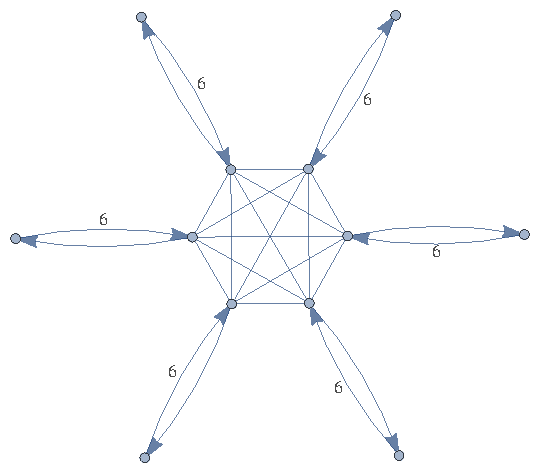
\includegraphics[width=0.3\textwidth]{K6WithGadgets}
  \end{figure}
  \begin{figure}[h!]
    \caption{The quotient graphs $\Gamma / H_1$ and $\Gamma / H_2$}\label{fig:SunadaQuotients}
    \centering
    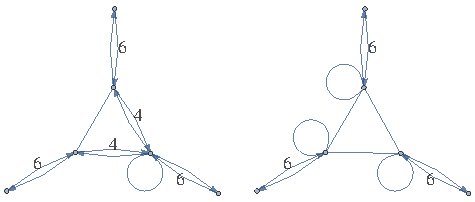
\includegraphics[width=0.5\textwidth]{SunadaQuotients}
  \end{figure}

  \begin{example}
    Here we demonstrate the extension of Sunada's theorem to orbigraphs by producing two non-isomorphic, cospectral orbigraphs as quotients of a larger orbigraph. The original orbigraph $\Gamma$ we will consider is shown in Figure \ref{fig:K6WithGadgets}. The orbigraph $\Gamma$ consists of $K_6$ with one additional vertex attached to each vertex. From this, we see that its automorphism group $G$ is isomorphic to $S_6$. The action of the following subgroups $H_1$ and $H_2$ of $S_6$ on $\Gamma$ produces the two quotient graphs $\Gamma / H_1$ and $\Gamma / H_2$ in Figure \ref{fig:SunadaQuotients}.
    \begin{align*}
      H_1 &= \{ (12)(34), (13)(24), (14)(23) \} \\
      H_2 &= \{ (12)(34), (12)(56), (34)(56) \}
    \end{align*}
    The subgroups $H_1$ and $H_2$ are Sunada equivalent [ref buser] and so by Theorem \ref{thm:Sunada}, the quotient graphs $\Gamma / H_1$ and $\Gamma / H_2$ are cospectral. A simple calculation shows that their spectra are
    $$
    \spec(\Gamma / H_1) = \spec(\Gamma / H_2) = \{ -3, -3, -1, 2, 2, 6 \}.
    $$
    They are clearly not isomorphic.
  \end{example}

  Seidel Switching is a method used to construct cospectral pairs. It has previously been used in undirected graphs, but there is very little literature on its use in directed graphs. Here we show that the method can be extended to construct cospectral orbigraphs. In its most basic form, Seidel switching produces a pair of cospectral graphs by making connections between two given graphs. 

  Suppose $\Gamma_1$ and $\Gamma_2$ are $k$-orbigraphs each on $2l$ vertices with adjacency matrices $A$ and $B$ respectively. Furthermore, suppose that $T$ is a \textbf{switching matrix}, that is, it is a $(0,1)$-matrix with each row and each column summing to $l$. Let $J$ be a $2l \times 2l$ matrix of ones. Then define two new orbigraphs $\mathcal{S}_1$ and $\mathcal{S}_2$ as follows:

  $$
  A(\mathcal{S}_1) = \begin{bmatrix}
      A & T \\
      T^T & B
  \end{bmatrix} \ \ 
  A(\mathcal{S}_2) = \begin{bmatrix}
      A & J - T \\
      (J - T)^T & B
  \end{bmatrix}.
  $$

  \begin{theorem}\label{thm:SeidelSwitchingSimple}
  The orbigraphs $A(\mathcal{S}_1)$ and $A(\mathcal{S}_2)$ as defined above are cospectral.
  \end{theorem}

  Remark: The standard method of proving this result [ref Brooks] relies on the fact that in an undirected graph, the number of walks of a given length originating at a given vertex is equal to the number of walks of that length terminating at the vertex. This is untrue for orbigraphs, so the well known proof is insufficient.

  \begin{lemma}\label{lemma:SwitchedPowers1}
    If $T$ is any switching matrix and $A$ and $B$ are as above, then 
    $$
      \begin{bmatrix}
        A & T \\\\
        T^T & B
      \end{bmatrix}^n = \begin{bmatrix}
        X & Y \\\\
        Z & W
      \end{bmatrix}
    $$ where $X, Y, Z$, and $W$ are constant row sum matrices and the row sums of each are independent of $T$.
\end{lemma}

\begin{proof} We will proceed by induction on $n$. The base case is trivial. Assume that for some $n = m$ the lemma holds. Then we have
  $$
    \begin{bmatrix}
      A & T \\\\
      T^T & B
    \end{bmatrix}^{m+1} = \begin{bmatrix}
      X & Y \\\\
      Z & W
    \end{bmatrix} \cdot \begin{bmatrix}
      A & T \\\\
      T^T & B
    \end{bmatrix} = \begin{bmatrix}
      XA + YT^T & ZA + WT^T \\\\
      XT + YB & ZT + WB
    \end{bmatrix}.
  $$
  Because each block is a sum of products of constant row sum matrices, they are constant row sum matrices themselves. Furthermore, to see that the row sum is independent of $T$, calculate i.e. $Rs(XA + YT^T) = Rs(X)Rs(A) + Rs(Y)Rs(T^T) = Rs(X)Rs(A) + Rs(Y) \cdot l$. Which is independent of $T$ by the induction hypothesis.
\end{proof}


\begin{lemma}\label{lemma:SwitchedPowers2}
  For any $n$, we have $A(\mathcal{S}_1)^n = \begin{bmatrix}
    C & X \\\\
    Y & D
  \end{bmatrix}$ and $A(\mathcal{S}_2)^n = \begin{bmatrix}
    C - S_1 & S_2 - X \\\\
    S_3 - Y & D - S_4
  \end{bmatrix}$, where $S_1,\ldots,S_4$ are constant column matrices, and $S_1$ and $S_4$ have row sums $0$.
\end{lemma}

\begin{proof} We will proceed by induction on $n$. For the base case, we let $C = A, X = T, Y = T^T, D = B, S_1 = 0, S_2 = J, S_3 = J, S_4 = 0$. The only thing interesting to note here is that $S_3 = J$ is valid because $S_3 - Y = J - T^T = (J - T)^T$, using the fact that $J$ is symmetric.

Now, suppose that for some $n = m$ the theorem holds. Then we have
$$
A(\mathcal{S}_1)^{m+1} = \begin{bmatrix}
    C & X \\\\
    Y & D
\end{bmatrix} \cdot \begin{bmatrix}
    A & T \\\\
    T^T & B
\end{bmatrix} = \begin{bmatrix}
    CA + XT^T & CT + XB \\\\
    YA + DT^T & YT + DB
\end{bmatrix}.
$$

Furthermore, we have

\begin{align*}
  A(\mathcal{S}_1)^{m+1} &= \begin{bmatrix}
      C - S_1 & S_2 - X \\
      S_3 - Y & D - S_4
  \end{bmatrix} \cdot \begin{bmatrix}
      A & J - T \\
      (J - T)^T & B
  \end{bmatrix} \\ &= \begin{bmatrix}
      (CA + XT^T) - S_1 A + S_2 J - S_2 T^T - X J & CJ - S_1 J + S_1 T + S_2 B - (CT + XB) \\\\
      S_3 A + DJ - S_4 J + S_4 T^T - (YA + DT^T) & (YT + DB) + S_3 J - S_3 T - YJ - S_4 B
  \end{bmatrix}
\end{align*}

Thus we now have
\begin{align*}
S'_1 &= - S_1 A + S_2 J - S_2 T^T - X J \\\\
S'_2 &= CJ - S_1 J + S_1 T + S_2 B \\\\
S'_3 &= S_3 A + DJ - S_4 J + S_4 T^T \\\\
S'_4 &= S_3 J - S_3 T - YJ - S_4 B
\end{align*}
We need only verify that these are each constant column matrices and that $Rs(S'_1) = Rs(S'_4) = 0$. To see that they are constant column matrices, note that each $S'_i$ is the sum of multiples of $S_j$ and left multiples of $J$ by constant row sum matrices. By the induction hypothesis, $S_j$ is a constant colum matrix, so any multiple thereof is as well. Furthermore, any left multiple of $J$ by a constant row sum matrix is a multiple of $J$ and is therefore a constant column matrix. Thus the $S'_j$ are constant column matrices. 

By the previous lemma, we have that $Rs(CA + XT^T - S'_1) = Rs(CA + XT^T)$, but this implies that $Rs(S'_1) = 0$. The same reasoning shows that $Rs(S'_4) = 0$.
\end{proof}

\begin{proof}[Proof of Theorem \ref{thm:SeidelSwitchingSimple}] The result follows immediatly from Lemma \ref{lemma:SwitchedPowers2} and Theorem \ref{thm:LengthSpectrum}. We have
$$
Tr(A(\mathcal{S}_2)^n) = Tr\begin{bmatrix}
    C - S_1 & S_2 - X \\\\
    S_3 - Y & D - S_4
\end{bmatrix} = Tr(C) - Tr(S_1) + Tr(D) - Tr(S_4).
$$
However, $S_1$ and $S_4$ are constant column matrices with row sums $0$, so their traces are $0$. Hence $Tr(A(\mathcal{S}_2)^n) = Tr(A(\mathcal{S}_1)^n)$.
\end{proof}


  Remark: This theorem can easily be extended to show a pair of cospectral covering orbigraphs can be generated for any orbigraph. (Proof is very similar, not sure we need to include it\ldots.)

  \begin{theorem}\label{thm:SeidelSwitchingExtension}
    Suppose $\Gamma$ is a $k$-orbigraph on $m$ vertices and $\cover{\Gamma}_1,\ldots,\cover{\Gamma}_m$ are $k_1,\ldots,k_n$-orbigraphs on $2n_1,\ldots,2n_m$ vertices such that $k_i = A(\Gamma)_{ii}$ and $s_{ij} = A(\Gamma)_{ij} / n_j$ is an integer. Then there exist switching matrices $T_{ij}$ such that the two orbigraphs 
    $$
    A(\mathcal{S}_1) = \begin{bmatrix}
      \cover{\Gamma}_1  & T_{12}            & \cdots & T_{1m} \\
      T_{21}            & \cover{\Gamma}_2  & \cdots & T_{2m} \\
      \vdots            & \vdots            & \ddots & \vdots \\
      T_{m1}            & T_{m2}            & \cdots & \cover{\Gamma}_m
    \end{bmatrix} \ \ 
    A(\mathcal{S}_1) = \begin{bmatrix}
      \cover{\Gamma}_1  & s_{12}J - T_{12}  & \cdots & s_{1m}J - T_{1m} \\
      s_{21}J - T_{21}  & \cover{\Gamma}_2  & \cdots & s_{2m}J - T_{2m} \\
      \vdots            & \vdots            & \ddots & \vdots \\
      s_{m1}J - T_{m1}  & s_{m2}J - T_{m2}  & \cdots & \cover{\Gamma}_m
    \end{bmatrix}
    $$
    are cospectral and cover $\Gamma$.
  \end{theorem}

  This gives a simple method of finding cospectral good and bad orbigraphs:

  \begin{corollary}\label{coro:GoodBadCospectral}
    There are cospectral good and bad orbigraphs.
  \end{corollary}
  \begin{proof}
    Let $\Gamma$ an orbigraph with adjacency matrix given by
    $$
    A(\Gamma) = 
      \left( \begin{array}{cc}
        1 & 2 \\
        1 & 2
      \end{array} \right).
    $$
    Constructing a pair of cospectral orbigraphs $S_1$ and $S_2$ by switching $\Gamma$ with itself using the switching matrix $I_2$. The adjacency matrices for $S_1$ and $S_2$ are:
    $$
    A(S_1) = 
      \bordermatrix {
            & v_1 & v_2 & v_3 & v_4 \cr
        v_1 & 1   & 2   & 1   & 0   \cr
        v_2 & 1   & 2   & 0   & 1   \cr
        v_3 & 1   & 0   & 1   & 2   \cr
        v_4 & 0   & 1   & 1   & 2
      } \ \ 
    A(S_2) = 
      \bordermatrix {
            & v_1 & v_2 & v_3 & v_4 \cr
        v_1 & 1   & 2   & 0   & 1   \cr
        v_2 & 1   & 2   & 1   & 0   \cr
        v_3 & 0   & 1   & 1   & 2   \cr
        v_4 & 1   & 0   & 1   & 2
      }.
    $$
    By inspection, we see that $S_1$ and $S_2$ each have only one non-trivial cycle. In $S_1$ this cycle is $v_1 v_2 v_4 v_3$ and there are $2$ ways to traverse this cycle in either direction. However, in $S_2$ the nontrivial cycle is $v_1 v_2 v_3 v_4$ and there are $4$ ways to traverse it forward, but only one way to traverse it in reverse. Hence by Theorem \ref{thm:GoodBadCharacterization}, $S_1$ is good, but $S_2$ is bad.
  \end{proof}


%%%%%%%%%%%%%%%%%%%%%%%%%%%%%%%%%%%%%%%%%%%%%%%%%%%%%%%
\section{Conclusion}
  Some concluding remarks.


%%%%%%%%%%%%%%%%%%%%%%%%%%%%%%%%%%%%%%%%%%%%%%%%%%%%%%%
\subsection*{Acknowledgements}
  Acknowledgements here.


%%%%%%%%%%%%%%%%%%%%%%%%%%%%%%%%%%%%%%%%%%%%%%%%%%%%%%%
% \bibliographystyle{plain} 
% \bibliography{myBibFile} 
% If you use BibTeX to create a bibliography
% then copy and past the contents of your .bbl file into your .tex file

\begin{thebibliography}{10}

\end{thebibliography}

\end{document}